\documentclass[a4paper,twoside,11pt, fleqn]{article}
\usepackage{a4wide,graphicx,fancyhdr,amsmath,amssymb}
\usepackage{listings}
\usepackage{color}
\usepackage{dirtree}
\usepackage{subcaption}

%matlab 
\usepackage[]{mcode}

%----------------------- Macros and Definitions --------------------------

\setlength\headheight{20pt}
\addtolength\topmargin{-10pt}
\addtolength\footskip{20pt}

\newcommand{\N}{\mathbb{N}}
\newcommand{\ch}{\mathcal{CH}}

\newcommand{\solution}[1]{\noindent{\bf Solution to Exercise #1:}}

\fancypagestyle{plain}{%
\fancyhf{}
\fancyhead[LO,RE]{\sffamily\bfseries\large technische universiteit eindhoven}
\fancyhead[RO,LE]{\sffamily\bfseries\large 2IN35 VLSI}
\fancyfoot[LO,RE]{\sffamily\bfseries\large department of mathematics and computer science}
\fancyfoot[RO,LE]{\sffamily\bfseries\thepage}
\renewcommand{\headrulewidth}{0pt}
\renewcommand{\footrulewidth}{0pt}
}

\pagestyle{fancy}
\fancyhf{}
\fancyhead[RO,LE]{\sffamily\bfseries\large technische universiteit eindhoven}
\fancyhead[LO,RE]{\sffamily\bfseries\large 2IN35 VLSI}
\fancyfoot[LO,RE]{\sffamily\bfseries\large department of mathematics and computer science}
\fancyfoot[RO,LE]{\sffamily\bfseries\thepage}
\renewcommand{\headrulewidth}{1pt}
\renewcommand{\footrulewidth}{0pt}

\def\addsquare#1{\tikz\node[draw]{#1};} 

%-------------------------------- Title ----------------------------------

\title{\vspace{-\baselineskip}\sffamily\bfseries Assignment 4}
\author{
	Rick Veens \qquad Studentno: 0912292\\
	\texttt{r.veens@student.tue.nl}
	\and
	Barry de Bruin \qquad Studentno: 0919605\\
	\texttt{e.d.bruin@student.tue.nl}
	\and
	\texttt{Group 7}
}

\date{\today}

\setlength\parindent{0pt}

%--------------------------------- Text ----------------------------------

\begin{document}
\maketitle
\newpage

\tableofcontents

\newpage
\section{Inline questions}
\subsection{Inline question 1}
The theoretical bound would be one cycle per output sample. The maximum number of streams would then be:\\

$max_{\# streams} = \dfrac{system\_frequency \cdot sample\_frequency}{\frac{cycles}{sample}} = \dfrac{100MHz \cdot 48KHz}{1} \approx 2083$ streams\\

\subsection{Inline question 2}
We waste two cycles to shift in one sample of data. Then we also use one cycle to make sure that the output acknowledge is received, and we use one cycle to calculate a sample. If we re-use the samples (due to upsampling), we will not use the two cycles to process the input.\\

Every 147 input samples, we produce 160 output samples. If we assume that the acknowledgement of input and output occurs the very next cycle after requesting (which is probably not very likely), the amount of cycles required to produce 160 samples is:
\begin{align*}
amount\_of\_cycles &= 147\cdot (2 + 1 + 1) + (160-147)\cdot (1  + 1 )\\
&= 588 + 26\\
&= 614
\end{align*}

This will result in: $\frac{614}{160} \approx 4$ cycles per sample. 

\subsection{Inline question 3}
Since we have 2083 clock cycles available, to produce all samples of one stream, and our design needs approximately 4 cycles to produce one output, our maximum output stream number is limited to $\frac{2083}{4} \approx 521$ streams.

\newpage
\section{System architecture}
Figure one shows the global architecture of the FIR filter. 
\begin{figure}[h]
	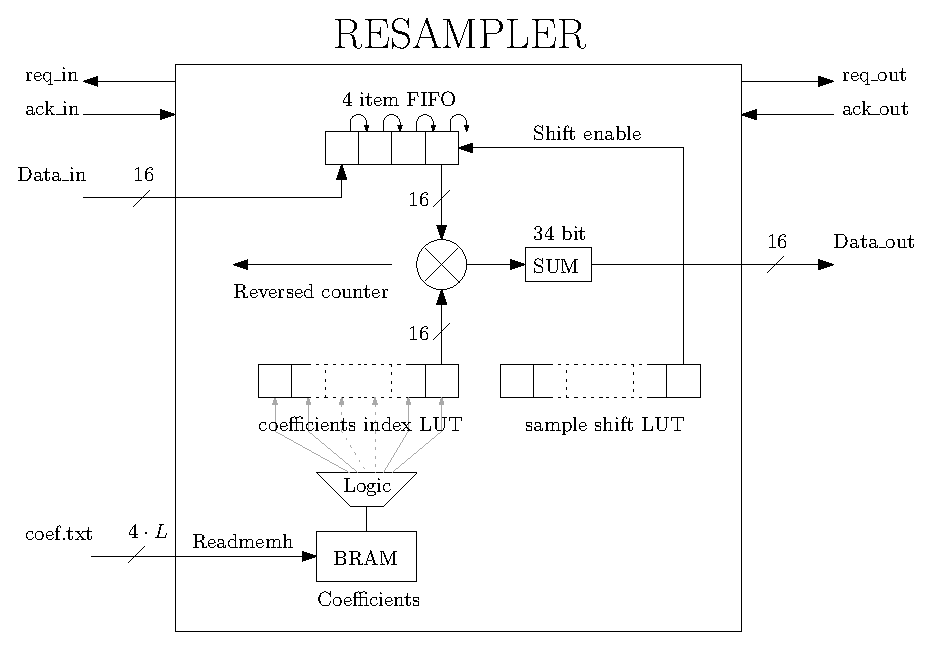
\includegraphics[scale = 0.85]{Images/5_blockdiagram}
    \caption{System overview}
\end{figure}

The resampler is an extension of the implementation of lab 4. The upper part has changed. We can see that four Block RAM modules are used to shift the data samples in.\\

Four DSP units are used to calculated one sample in one cycle. Because of the fact that all these steps are pipelined, we needed to have a stream delay buffer. This stream delay buffer delays the calculated samples one full stream-length minus the additional delay of the calculation pipeline. This ensures that a full stream of samples, is not shifted, but delayed one full stream length.

\newpage
\section{Design choices}

\newpage
\section{Resource usage}
Table~\ref{tab:3ausage} summarizes the resources used by the multi-stream resampler. This list is obtained by running the synthesis step in Xilinx ISE and extracted from the \textit{Summary} and \textit{Device Utilization} report.

\begin{table}[h]
\begin{tabular}{|l|l|l|l|}
\hline
\textbf{Resource} & \textbf{Available} & \textbf{Utilized} & \textbf{Percentage utilized}\\
\hline
Flip Flops	& 54576 & 70 	& 1\%\\
Slice LUTs 	& 27288 & 212 	& 1\%\\
DSP48A1s	& 58 	& 4 	& 6\%\\
BRAM		& 116 	& 2 	& 1\%\\
Bonded IOBs	& 218 	& 38	& 17\%\\
\hline
\end{tabular}
\caption{General resource usage overview}
\label{tab:3ausage}
\end{table} 

4 DSP units are used, since one sample is calculated in one clock cycle, by using the direct form equation.\\

Both the coefficient index and shift enable LUT are stored in DRAM. This because they are both read-only. \\

We tried to use BRAM for our ram modules. They are also shown als Block RAM in our block diagram. However, the compiler has actually not synthesized them as BRAMs but as LUTs. This has probably to do that we did not buffer the output of the RAM, which makes it asynchronous.\\

The compiler did create block ram for the delay buffer. This buffer uses $NR\_STREAMS * DDWIDTH$ bits.

\newpage
\section{System throughput and latency}
The synthesis estimation is as follows:\\

\textit{Minimum period: 6.164ns (Maximum Frequency: 162.234MHz)\\
Minimum input arrival time before clock: 5.080ns\\
Maximum output required time after clock: 3.820ns}\\

After doing the placement and routing step, we get the following timing summary:\\

\textit{Minimum period:   7.528ns{1}   (Maximum frequency: 132.837MHz)\\
Minimum input required time before clock:   4.323ns\\
Maximum output delay after clock:   8.707ns}\\

Since the maximum delay is below 10ns, we can be sure that our design is able to run at 100MHz. Our maximum clock frequency, according to the \textit{Advanced Post-PAR static timing report} under \textit{Timing summary}, is: $\dfrac{1}{8.708ns} \approx 115MHz$. 
   
\newpage
\section{Offline project results}
\subsection{256 Streams}
\subsection{1024 Streams}

\newpage
\section{Appendix A: Matlab coefficients script}
\begin{lstlisting}
% Put this in a file named coef_generate_matlab.m, then call it 
% while you are in the file directory. It will write the coefficients
% to the coef.txt file and also return them.

function [y] = coef_generate_matlab(L)
        % make sure that coefficients sum to 1
        y = coef_gen(L);
        y = y/sum(y);

        % quantize and round to nearest integer
        y = y * 160;
        y = round(y*(2^15)); 
             
        % convert to signed int filter coeff
        y = int16(y);
        y = hex(fi(y, 1, 16, 0)); %1 stands for signed, 16 bit out
        
        dlmwrite('coef.txt',y,''); %create file, with no delimiter ''      
end

function [y] = coef_gen(L)
    % generate 4*L coefficients and start at 0 instead of 1 *stupid matlab*
    for n = 1:4*L
            y(n) = lanczos2(((n-1)/L) -2);
    end
end

function y = lanczos2(t)
    if(t <= -2 || t >= 2)
        y = 0;
    else
        y = sinc(t).*sinc(t/2);
    end
end
\end{lstlisting}

Figure~\ref{fig:frq} shows the frequency response of the FIR filter that is generated with help of the matlab code from appendix A.

\begin{figure}[h]
	\includegraphics[scale=0.67]{Images/frequencyplot}
    \caption{Interpolation filter frequency domain (Matlab)}
    \label{fig:frq}
\end{figure}

\newpage
\section{Appendix B: Verilog Code}
File: filter.v.
\begin{lstlisting}[language=Verilog]

\end{lstlisting}

\end{document}
